\documentclass[
	12pt,
	openright,
	oneside,
	a4paper,
	english,
	brazil
	]{abntex2}

% ---
% PACOTES BÁSICOS
% ---
\usepackage{lmodern}
\usepackage[T1]{fontenc}
\usepackage[utf8]{inputenc}
\usepackage{indentfirst}
\usepackage{color}
\usepackage{graphicx}
\usepackage{microtype}
\usepackage{amsmath}
\usepackage{listings}
\usepackage{xcolor}
\usepackage{url}
\usepackage{booktabs}
\usepackage{float}
\usepackage{subcaption}
\usepackage[alf]{abntex2cite}

% Configuração de código-fonte
\lstset{
  basicstyle=\footnotesize\ttfamily,
  breaklines=true,
  frame=single,
  captionpos=b,
  language=Python,
  keywordstyle=\color{blue},
  commentstyle=\color{gray},
  stringstyle=\color{red},
}

% ---
% INFORMAÇÕES DO TRABALHO
% ---
\titulo{Filtro de Dados e Compressão para Computação em Névoa em IoT na Agricultura Inteligente utilizando Rust e WebAssembly}
\autor{Victor Cobo}
\local{Santo André}
\data{2026}
\orientador{Prof. Dr. Carlos Alberto Kamienski}
\instituicao{%
  UNIVERSIDADE FEDERAL DO ABC
  \par
  CMCC -- CENTRO DE MATEMÁTICA, COMPUTAÇÃO E COGNIÇÃO
  \par
  BACHARELADO EM CIÊNCIA DA COMPUTAÇÃO}
\tipotrabalho{Projeto de Graduação em Computação}
\preambulo{Projeto de Graduação em Computação apresentado ao Bacharelado em Ciência da Computação da Universidade Federal do ABC, como requisito parcial para a obtenção do título de Bacharel.}

% ---
% CONFIGURAÇÕES DE APARÊNCIA E CAPA
% ---
\definecolor{blue}{RGB}{41,5,195}
\hypersetup{
    pdftitle={\@title},
    pdfauthor={\@author},
    pdfsubject={\imprimirpreambulo},
    colorlinks=true,
    linkcolor=black,
    citecolor=black,
    urlcolor=black
}

\renewcommand{\imprimircapa}{%
  \begin{capa}%
    \centering
    \vspace*{1cm}
    
\includegraphics[width=4cm]{Ufabc_logo.png} \\
    \vspace{0.5cm}
    {\ABNTEXchapterfont\large\imprimirinstituicao}
    
    \vspace*{\fill}
    
    {\ABNTEXchapterfont\large\imprimirautor}
    
    \vspace*{\fill}
    
    {\ABNTEXchapterfont\bfseries\LARGE\imprimirtitulo}
    
    \vspace*{\fill}
    
    {\large\imprimirlocal}
    \par
    {\large\imprimirdata}
    \vspace*{1cm}
  \end{capa}
}

% ---
% INÍCIO DO DOCUMENTO
% ---
\begin{document}

\selectlanguage{brazil}
\frenchspacing

% ----------------------------------------------------------
% ELEMENTOS PRÉ-TEXTUAIS
% ----------------------------------------------------------
\imprimircapa
\imprimirfolhaderosto

% --- Dedicatória ---
\begin{dedicatoria}
   \vspace*{\fill}
   \centering
   \noindent
   \textit{Dedico este trabalho à minha família pelo apoio incondicional, aos meus colegas de curso pelas noites de estudo compartilhadas, e a todos que enxergam na computação uma ferramenta para transformar a interação humana com o meio ambiente.}
   \vspace*{\fill}
\end{dedicatoria}

% --- Agradecimentos ---
\begin{agradecimentos}
Agradeço primeiramente ao meu orientador, Prof. Dr. Carlos Alberto Kamienski, pelo suporte técnico, paciência e pelas valiosas discussões acadêmicas ao longo do desenvolvimento deste projeto. Agradeço à Universidade Federal do ABC pelo ensino público de excelência e a todos os professores que contribuíram para minha formação científica. Por fim, aos meus amigos e familiares, cujo encorajamento foi essencial nesta jornada.
\end{agradecimentos}

% --- Epígrafe ---
\begin{epigrafe}
    \vspace*{\fill}
	\begin{flushright}
		\textit{``A tecnologia é apenas uma ferramenta. No que diz respeito a fazer as crianças trabalharem juntas e motivá-las, o professor é o mais importante.''\\
		(Bill Gates)}
	\end{flushright}
\end{epigrafe}

% --- Resumo ---
\begin{resumo}
A agricultura inteligente é uma das principais fronteiras da Internet das Coisas (IoT), exigindo o monitoramento de variáveis físicas contínuas em ambientes remotos. Contudo, a transmissão em tempo real de grandes volumes de dados de sensores para a nuvem por canais de baixa potência e banda restrita (como LoRaWAN) gera alta latência, congestionamento e rápido esgotamento energético dos dispositivos. Este trabalho propõe e avalia um ecossistema de computação em névoa baseado em Rust e WebAssembly (WASM) para realizar filtragem e compressão de dados na borda da rede. Utilizando o algoritmo de classificação $k$-Vizinhos Mais Próximos ($k$NN, com $k=3$) adaptado para as condições agronômicas de cultivo do tomateiro, o sistema converte medidas físicas contínuas de temperatura e umidade em status discretos de um caractere, os quais são posteriormente comprimidos via Run Length Encoding (RLE). Para a validação estatística, implementou-se um gerador de dados estocásticos via Estimativa de Densidade por Kernel (KDE) e Transformada de Box-Muller nativamente em Rust/WASM. Os experimentos compararam a base original (\texttt{entrada.csv}, com 44.023 registros) e amostras sintéticas de 40.000 pontos em três execuções independentes. O gerador em Rust demonstrou altíssima fidelidade estatística, validada pelo teste de Kolmogorov-Smirnov (p-valor de $0,1385$ para temperatura e $0,8974$ para umidade) e pelo desvio de correlação de Pearson de apenas $0,0033$. Os resultados mostraram que o kNN isolado alcança $97,84\%$ de redução de volume de dados (reduzindo a base para 40 KB), superando a combinação kNN+RLE ($96,32\%$, ou 68 KB). Isso revela a ineficiência do RLE em alfabetos curtos de caractere único frente à variabilidade natural de alta frequência dos sensores físicos, fornecendo diretrizes de projeto cruciais para arquiteturas de IoT na névoa.

\textbf{Palavras-chave}: Computação em Névoa. Internet das Coisas (IoT). Agricultura Inteligente. Rust. WebAssembly. WasmEdge. Compressão de Dados.
\end{resumo}

% --- Abstract ---
\begin{resumo}[Abstract]
\begin{otherlanguage*}{english}
Smart agriculture stands as one of the primary frontiers for the Internet of Things (IoT), requiring continuous monitoring of environmental variables in remote areas. However, streaming large volumes of raw sensor data directly to the cloud over low-power, narrow-bandwidth channels (such as LoRaWAN) causes network congestion, latency, and rapid battery depletion. This work proposes and evaluates a fog computing ecosystem built with Rust and WebAssembly (WASM) to perform data filtering and compression at the network edge. Using a $k$-Nearest Neighbors classification algorithm ($k$NN, with $k=3$) tailored to tomato agronomic status, the system maps continuous temperature and humidity readings into single-character discrete labels, which are compressed using Run Length Encoding (RLE). For validation, an offline stochastic data generator was developed natively in Rust/WASM using Kernel Density Estimation (KDE) and the Box-Muller transform. Experiments compared the original dataset (\texttt{entrada.csv}, 44,023 records) with synthetic samples of 40,000 points across three independent runs. The Rust generator achieved high statistical fidelity, validated by the Kolmogorov-Smirnov test (p-value of $0.1385$ for temperature and $0.8974$ for humidity) and a Pearson correlation deviation of just $0.0033$. Results showed that standalone $k$NN achieves a $97.84\%$ data reduction (shrinking the payload to 40 KB), outperforming the combined $k$NN+RLE approach ($96.32\%$, or 68 KB). This highlights the inefficiency of RLE when applied to a single-character alphabet under high-frequency physical sensor fluctuations, providing critical design guidelines for fog-based IoT architectures.

\vspace{\onelineskip}
\noindent
\textbf{Keywords}: Fog Computing. Internet of Things (IoT). Smart Agriculture. Rust. WebAssembly. WasmEdge. Data Compression.
\end{otherlanguage*}
\end{resumo}

% --- Listas ---
\pdfbookmark[0]{\listfigurename}{lof}
\listoffigures*
\cleardoublepage

\pdfbookmark[0]{\listtablename}{lot}
\listoftables*
\cleardoublepage

% --- Sumário ---
\pdfbookmark[0]{\contentsname}{toc}
\tableofcontents*
\cleardoublepage

% ----------------------------------------------------------
% ELEMENTOS TEXTUAIS
% ----------------------------------------------------------
\textual

% ==========================================================
\chapter{INTRODUÇÃO}
% ==========================================================

A Internet das Coisas (IoT) revolucionou a agricultura de precisão, permitindo que sensores coletem continuamente variáveis ambientais como temperatura, umidade, luminosidade e umidade do solo. Na agricultura inteligente, o monitoramento em tempo real dessas grandezas é vital para otimizar a produtividade e a saúde das plantações. No entanto, a arquitetura tradicional que centraliza a coleta de dados e os envia diretamente à nuvem enfrenta graves gargalos operacionais.

Sensores implantados no campo operam sob fortes restrições de energia e dependem de redes de comunicação sem fio de baixa potência e longo alcance (LPWAN), como LoRaWAN, que operam com taxas de transmissão extremamente baixas (tipicamente entre 292 bps e 50 kbps) e limitações rígidas de ciclo de trabalho (\textit{duty cycle}). O envio ininterrupto de dados brutos gera alto consumo de bateria nos nós sensores e congestionamento de rede no gateway.

Nesse cenário, a computação em névoa (\textit{fog computing}) atua como uma camada intermediária entre os dispositivos sensores de borda e os servidores em nuvem. Ao transferir capacidade computacional de processamento e tomada de decisão para os gateways locais, torna-se possível aplicar algoritmos de filtragem de dados e compressão antes da transmissão WAN. Desta forma, envia-se apenas informação relevante para a nuvem, economizando largura de banda e prolongando a vida útil das baterias dos nós de borda.

\section{PROBLEMA DE PESQUISA}

A filtragem de dados na névoa exige um ambiente de execução leve, portável e seguro para rodar códigos de terceiros nos gateways de borda. Máquinas virtuais pesadas ou contêineres tradicionais (como Docker) demandam muitos recursos computacionais, tornando-se inviáveis para os hardwares limitados comuns na névoa. Além disso, linguagens tradicionais de script (como Python) carecem do desempenho e eficiência necessários, enquanto linguagens compiladas nativas (como C/C++) apresentam riscos severos de segurança de memória.

A pesquisa original de \cite{ribeiro2020nearest} propôs o uso de $k$-Vizinhos Mais Próximos ($k$NN) e Run Length Encoding (RLE) em gateways para reduzir a taxa de transmissão em aplicações agrícolas. Contudo, a viabilização prática desse modelo em sistemas de produção exige responder à seguinte questão: \textit{Como implementar e validar um ecossistema seguro, portável e de alto desempenho para filtragem e compressão de dados agrícolas na borda, utilizando modernas tecnologias de compilação como Rust e WebAssembly, e como garantir a estabilidade e a validade estatística desse processamento em cenários off-line?}

\section{OBJETIVOS}

\subsection{Objetivo Geral}

Propor, implementar e validar um framework fim-a-fim de computação em névoa que realiza filtragem de dados agronômicos por meio de classificação $k$NN e compressão RLE, compilado para WebAssembly (WASM) a partir de Rust e executado no ambiente de alto desempenho WasmEdge.

\subsection{Objetivos Específicos}

\begin{itemize}
    \item Implementar o classificador $k$NN ($k=3$) para classificar dados de sensores em 11 classes de sanidade do tomateiro;
    \item Desenvolver o codificador RLE em Rust para comprimir sequências de classes resultantes do kNN;
    \item Desenvolver um módulo de simulação estocástica de dados nativo em Rust que implementa Estimativa de Densidade por Kernel (KDE) e Transformada de Box-Muller para ambiente WASM/WASI;
    \item Validar estatisticamente a fidelidade do gerador estocástico contra a base de dados reais de sensores (\texttt{entrada.csv}) por meio de testes de Kolmogorov-Smirnov (KS-test) e correlação de Pearson;
    \item Avaliar comparativamente a eficiência de compressão obtida com kNN isolado e kNN+RLE sob diferentes tamanhos de lote de processamento.
\end{itemize}

\section{JUSTIFICATIVA}

A transposição de algoritmos de processamento de dados para a névoa usando a linguagem Rust e o ambiente WebAssembly justifica-se por razões tecnológicas e práticas fundamentais:

\textbf{Desempenho e Segurança}: Rust garante segurança de memória sem a necessidade de um coletor de lixo (\textit{garbage collector}), entregando eficiência equivalente a C/C++ sem o risco de falhas catastróficas (\textit{buffer overflows}, vazamento de memória).

\textbf{Portabilidade e Isolamento}: WebAssembly fornece um \textit{sandbox} seguro e leve que permite rodar código compilado quase na velocidade nativa, independente do processador (ARM, x86) ou do sistema operacional do gateway de névoa.

\textbf{Economia de Infraestrutura}: A redução sistemática do tamanho dos pacotes e da frequência de envio viabiliza a implantação de um número maior de sensores sob a mesma infraestrutura LoRaWAN existente.

\textbf{Validação Estatística com Dados Sintéticos}: A capacidade de gerar dados sintéticos estatisticamente idênticos permite testar de forma robusta e exaustiva novos algoritmos e configurações de rede off-line, sem a necessidade de dispendiosas campanhas de campo para coleta contínua.

\section{DISCIPLINAS FORMADORAS DO PROJETO}

O desenvolvimento do projeto utilizou conceitos de diversas áreas de conhecimento da Ciência da Computação da UFABC, conforme detalhado na Tabela~\ref{tab:disciplinas}.

\begin{table}[H]
\centering
\caption{Disciplinas do BCC/UFABC e sua contribuição ao projeto}
\label{tab:disciplinas}
\resizebox{\textwidth}{!}{%
\begin{tabular}{|p{5.5cm}|p{3.5cm}|p{7.5cm}|}
\hline
\textbf{Disciplina} & \textbf{Código} & \textbf{Contribuição ao Projeto} \\ \hline

Inteligência Artificial & MCTA014-15 &
Fundamentação de classificadores supervisionados para a concepção e parametrização do algoritmo $k$NN. \\ \hline

Probabilidade e Processos Estocásticos & MCZA006-13 &
Fundamentação estatística para a implementação de modelos de densidade contínuos baseados em Kernel (KDE) e na transformação de Box-Muller. \\ \hline

Sistemas Distribuídos & MCTA025-13 &
Comunicação cliente-servidor e arquitetura de dados IoT na passagem de dados de sensores do Thing para a Névoa e para a Nuvem. \\ \hline

Redes de Computadores & MCTA024-13 &
Conhecimentos sobre protocolos de comunicação de baixo consumo e restrições de transmissão em canais sem fio de longa distância. \\ \hline

Compiladores & MCTA009-17 &
Compreensão da geração de representação intermediária e otimização de código necessária para compilar código Rust em bytecode WebAssembly. \\ \hline

Algoritmos e Estruturas de Dados II & MCTA002-17 &
Estruturas de representação na memória para busca de vizinhos mais próximos e indexação de buffer de dados temporais para compressão RLE. \\ \hline

\end{tabular}%
}
\fonte{O Autor (2026)}
\end{table}

\section{ORGANIZAÇÃO DO TEXTO}

Este trabalho está estruturado da seguinte forma: o Capítulo~\ref{cap:referencial} apresenta o referencial teórico cobrindo as tecnologias Rust, WebAssembly, kNN, RLE e o gerador estocástico; o Capítulo~\ref{cap:revisao} detalha a revisão de literatura com foco no artigo MetroAGriFor 2020; o Capítulo~\ref{cap:desenvolvimento} descreve a arquitetura e implementação dos componentes; o Capítulo~\ref{cap:metodologia} apresenta a metodologia de teste e o plano de validação; o Capítulo~\ref{cap:resultados} discute os resultados obtidos, acompanhados das análises estatísticas e dos gráficos; e o Capítulo~\ref{cap:conclusao} resume as principais conclusões e propostas para trabalhos futuros.

% ==========================================================
\chapter{REFERENCIAL TEÓRICO}
\label{cap:referencial}
% ==========================================================

\section{Computação em Névoa (Fog Computing)}

A computação em névoa estende o paradigma da computação em nuvem para a borda da rede de modo a mitigar a latência e o consumo de banda. Em contraste com a nuvem, a névoa oferece recursos descentralizados com localização geográfica distribuída e proximidade física com os dispositivos IoT. Em sistemas agrícolas, os gateways locais (como Raspberry Pi ou gateways industriais) atuam como nós de névoa, realizando o processamento preliminar de leituras de sensores antes de encaminhá-las aos servidores de aplicação remotos.

\section{Rust e WebAssembly (WASM)}

\subsection{Linguagem Rust}

Rust é uma linguagem de programação focada em segurança, velocidade e concorrência. Seu sistema de tipos e o conceito de posse (\textit{ownership}) com checagem de tempo de vida (\textit{borrow checker}) eliminam erros comuns de gerência de memória em tempo de compilação, sem depender de coleta de lixo. Isso garante um consumo de memória previsível e baixo, ideal para os dispositivos de borda.

\subsection{WebAssembly (WASM) e WASI}

WebAssembly é um formato de instrução binária projetado para ser executado de forma portável em uma máquina virtual baseada em pilha. Embora originalmente concebido para navegadores web, o WASM expandiu-se para o lado do servidor por meio da \textit{WebAssembly System Interface} (WASI), que padroniza o acesso a recursos do sistema operacional (como arquivos, rede e relógio). O bytecode WASM é executado sob isolamento completo (\textit{sandbox}), protegendo o gateway hospedeiro contra códigos maliciosos ou falhas de execução.

\subsection{WasmEdge Runtime}

WasmEdge é um interpretador e compilador JIT/AOT de WebAssembly de alto desempenho otimizado para cenários de computação de borda, névoa e microsserviços. Desenvolvido sob a tutela da Cloud Native Computing Foundation (CNCF), ele suporta a especificação WASI e oferece extensões para acelerar inferência de redes neurais, tornando-o o runtime ideal para executar pipelines de processamento estocástico e classificação local.

\section{Algoritmo dos k-Vizinhos Mais Próximos (kNN)}

O $k$NN é um algoritmo de aprendizado supervisionado não-paramétrico. O princípio consiste em classificar um novo ponto no espaço tridimensional ou bidimensional a partir do voto majoritário dos seus $k$ vizinhos mais próximos no conjunto de treino.

Para que variáveis físicas com ordens de grandeza distintas (como temperatura em ${}^\circ\text{C}$ e umidade em $\%$) tenham o mesmo peso no cálculo das distâncias, aplica-se a normalização Min-Max dos dados para o intervalo $[0, 1]$ com base nos limites $x_{min}$ e $x_{max}$ obtidos a priori:
\begin{equation}
x_{norm} = \frac{x - x_{min}}{x_{max} - x_{min}}
\end{equation}

A distância Euclidiana entre um vetor de leitura de sensor $P = (T_p, H_p)$ e um ponto do conjunto de treinamento $Q = (T_q, H_q)$ no espaço normalizado bidimensional é dada por:
\begin{equation}
d(P, Q) = \sqrt{(T_{p,norm} - T_{q,norm})^2 + (H_{p,norm} - H_{q,norm})^2}
\end{equation}

O algoritmo seleciona os $k$ registros de treinamento com as menores distâncias $d$ e realiza uma votação majoritária para determinar a classe agronômica a ser associada à nova leitura física.

\section{Compressão Run Length Encoding (RLE)}

A codificação de comprimento de corrida (RLE) é um método simples de compressão de dados sem perdas (\textit{lossless}), ideal para sequências com repetições frequentes de símbolos idênticos. O algoritmo substitui sequências contíguas de um mesmo caractere por um par constituído pelo número de ocorrências e o próprio caractere (exemplo: a cadeia \texttt{AAAAABBB} é representada por \texttt{5A3B}). 

Em dados agrícolas classificados por kNN, a redundância temporal é elevada, uma vez que a temperatura e a umidade mudam lentamente, gerando longas corridas consecutivas do mesmo status agronômico (por exemplo, várias horas consecutivas no estado "Optimal").

\section{Geração Estocástica via KDE e Box-Muller}

\subsection{Estimativa de Densidade por Kernel (KDE)}

O KDE é um método não-paramétrico para estimar a função de densidade de probabilidade (PDF) de uma variável aleatória contínua multivariada. Dada uma amostra real $\{X_1, X_2, \dots, X_n\}$ extraída da base física, o estimador de densidade por kernel em $d$ dimensões é definido como:
\begin{equation}
\hat{f}(x) = \frac{1}{n h^d} \sum_{i=1}^n K\left(\frac{x - X_i}{h}\right)
\end{equation}
onde $h > 0$ é a largura de banda (\textit{bandwidth}) e $K(u)$ é a função de kernel gaussiano normal multivariado.

Para gerar um novo ponto sintético $x_{sint} = (T_{sint}, H_{sint})$ a partir do KDE:
\begin{enumerate}
    \item Seleciona-se uniformemente ao acaso um ponto base $X_i = (T_i, H_i)$ do conjunto de dados reais (\texttt{entrada.csv});
    \item Adiciona-se ruído normal independente de média $0$ e desvio padrão igual à largura de banda $h = 0.5$ em cada dimensão:
    \begin{align}
    T_{sint} &= T_i + Z_1 \cdot h \\
    H_{sint} &= H_i + Z_2 \cdot h
    \end{align}
    onde $Z_1, Z_2 \sim \mathcal{N}(0, 1)$ são variáveis aleatórias normais padrão independentes.
\end{enumerate}

\subsection{Transformada de Box-Muller}

A geração de variáveis normais padrão $Z \sim \mathcal{N}(0,1)$ em Rust dentro do sandbox WebAssembly (WASI) requer um algoritmo autossuficiente e determinístico. A transformada de Box-Muller converte duas variáveis pseudo-aleatórias mutuamente independentes distribuídas uniformemente no intervalo aberto $(0, 1]$, denotadas por $U_1$ e $U_2$, em duas variáveis normais padrão independentes:
\begin{align}
Z_0 &= \sqrt{-2 \ln(U_1)} \cdot \cos(2\pi U_2) \\
Z_1 &= \sqrt{-2 \ln(U_1)} \cdot \sin(2\pi U_2)
\end{align}
Esse método permite gerar o ruído estocástico gaussiano do KDE de forma exata e rápida sem recorrer a bibliotecas de sistema operacional ausentes no sandbox do WASM.

% ==========================================================
\chapter{REVISÃO DE LITERATURA}
\label{cap:revisao}
% ==========================================================

\section{Trabalho de Base: Ribeiro Junior et al. (2020) - MetroAGriFor 2020}

Este projeto baseia-se diretamente na metodologia proposta por \cite{ribeiro2020nearest}, intitulada \textit{"A Nearest Neighbors based Data Filter for Fog Computing in IoT Smart Agriculture"}. Aquele artigo estabeleceu as bases teóricas de um filtro de dados inteligente instalado em gateways de névoa locais.

No trabalho original, o filtro opera sobre sensores de temperatura e umidade aplicados à cultura de tomateiro. Para tal, as condições da planta são categorizadas de acordo com parâmetros agronômicos de estresse hídrico e térmico, gerando dados discretos que representam os estados de "Optimal", "Marginal", "Upper Fail", entre outros. O classificador $k$NN em nível de gateway é encarregado de mapear as variáveis físicas contínuas para essas classes discretas.

A proposta de Ribeiro Junior et al. demonstrou que, ao invés de transmitir as leituras flutuantes originais com alta frequência para a nuvem, a transmissão de sequências compactas de classes reduz sensivelmente o payload do protocolo de transporte (como MQTT ou HTTP sobre redes de satélite ou LoRa). A aplicação de compressão de corrida RLE sobre a cadeia de símbolos gerada pelo kNN estende essa redução ao compactar repetições temporais contíguas.

\section{Avanços Introduzidos pelo Presente Projeto}

Embora cientificamente elegante, o projeto original de \cite{ribeiro2020nearest} foi concebido de forma puramente teórica e avaliado localmente via scripts de simulação offline (MATLAB/Python). O presente trabalho promove os seguintes avanços metodológicos e de engenharia de software:

\begin{enumerate}
    \item \textbf{Mudança de Tecnologia}: Migração completa dos algoritmos de classificação kNN e codificação RLE para código Rust compilado para alvos WebAssembly (\texttt{wasm32-wasi}). Isso garante que a filtragem possa ser implantada de forma leve e segura em gateways reais sob o runtime WasmEdge;
    \item \textbf{Concepção do Modo Offline com Geração KDE}: Implementação de um gerador estocástico nativo em Rust que opera sob as restrições WASI. Isso permite aos operadores de gateways emular dados sintéticos com base em um arquivo original sem a necessidade de manter o sensor físico acoplado durante fases de calibração;
    \item \textbf{Avaliação Célula de Lote Estrita}: Teste do impacto prático de diferentes limites temporais de buffers (de 6 a 20.000 pacotes) para analisar as características reais de latência e ganho de compressão do RLE em escala temporal de produção.
\end{enumerate}

% ==========================================================
\chapter{DESENVOLVIMENTO E ARQUITETURA}
\label{cap:desenvolvimento}
% ==========================================================

\section{Visão Geral da Arquitetura}

O ecossistema implementado divide-se em quatro componentes principais distribuídos de forma a simular um ambiente de IoT real:

\begin{figure}[H]
\centering

\includegraphics[width=12cm]{Ufabc_logo.png} 
\caption{Esquema lógico do pipeline: Sensor $\to$ Névoa (WasmEdge kNN+RLE) $\to$ Nuvem}
\label{fig:diagrama_blocos}
\fonte{O Autor (2026)}
\end{figure}

\begin{enumerate}
    \item \textbf{Dispositivo IoT (Thing/Simulador)}: Simula os nós sensores de campo. Ele lê dados brutos do ambiente (ou dados sintéticos KDE) e transmite via protocolo local para o gateway;
    \item \textbf{Gateway de Névoa (LoRa Relay e Processador)}: Executa o runtime WasmEdge. O processador em Rust/WASM lê as variáveis físicas do buffer de entrada, normaliza os valores, classifica cada ponto pelo kNN ($k=3$) e codifica sequencialmente via RLE, armazenando os resultados locais de compressão;
    \item \textbf{Cloud Receiver (Nuvem)}: Recebe os dados processados e comprimidos do gateway, realiza a descompressão e armazena-os na base persistente para visualização do usuário.
\end{enumerate}

\section{Componentes do Código e Implementação}

A arquitetura de software do projeto foi desenvolvida utilizando a linguagem Rust, visando alto desempenho, segurança de memória e facilidade de portabilidade. O ecossistema é composto por três programas principais localizados nos diretórios do projeto:

\subsection{Dispositivo IoT (simulador)}
O módulo \texttt{simulador} emula a coleta física dos sensores de temperatura e umidade da cultura de tomateiro. Ele é configurado para realizar requisições HTTP do tipo \texttt{POST} para o gateway de névoa, enviando a leitura no formato JSON.

\subsection{Processador na Névoa (processador)}
O módulo \texttt{processador} é o núcleo do ecossistema. Ele é compilado para WebAssembly (\texttt{wasm32-wasi}) e executado sobre o runtime leve \texttt{WasmEdge}. Ele implementa:
\begin{itemize}
    \item A leitura e parsing das estruturas JSON correspondentes aos sensores;
    \item A base de dados de treinamento estática de 11 faixas de saúde do tomateiro;
    \item A normalização Min-Max e o algoritmo de busca e classificação de vizinhos $k$NN ($k=3$);
    \item O algoritmo de compressão Run-Length Encoding (RLE) temporal sobre a sequência de caracteres obtidos;
    \item Um gerador estocástico multivariado de dados sintéticos via KDE com ruído gaussiano (Box-Muller).
\end{itemize}

\subsection{Receptor na Nuvem (receiver)}
O módulo \texttt{receiver} atua como o servidor na nuvem que recebe as strings compactadas do processador, simula a descompressão dos dados de controle e realiza a escrita dos logs de recepção em um arquivo persistente (\texttt{monitoramento.txt}) para auditoria e exibição.

\section{Fluxos de Execução do Processador}

O processador foi projetado com suporte a dois fluxos operacionais principais que atendem a cenários de rede distintos:

\subsection{Modo Normal (Online / Serviço HTTP)}
Neste modo, o processador atua como um servidor HTTP ativo escutando por requisições de sensores em tempo real. Ele expõe a rota \texttt{POST /inserir} para coletar leituras contínuas. Em segundo plano, uma rotina assíncrona (\textit{background thread}) rodando a cada 30 segundos agrupa os dados acumulados, executa a compactação RLE, envia os dados comprimidos para o receptor na nuvem (\texttt{POST /receber}) e limpa o buffer local para o próximo ciclo de monitoramento.

\subsection{Modo Lote (Offline / Batch Mode)}
Ativado pela passagem do argumento posicional \texttt{batch} na CLI, este fluxo destina-se ao processamento local de arquivos de sensores para campanhas offline e avaliações científicas de longa duração. Ele lê diretamente um arquivo CSV de entrada (ex.: \texttt{entrada.csv}), divide os dados em lotes com base em um tamanho de pacote configurável (via flag \texttt{--tamanho-pacote}), executa a classificação kNN e compressão RLE para cada lote, exporta estatísticas agregadas completas no formato JSON (\texttt{estatisticas\_compressao.json}) e finaliza a execução.

\subsection{Modo de Geração de Dados Sintéticos}
Quando a flag \texttt{--synthetic} (ou \texttt{--sintetico}) é especificada em conjunto com o modo \texttt{batch}, o processador executa a amostragem baseada na Estimativa de Densidade por Kernel (KDE) a partir do CSV de referência. Ele gera 40.000 registros sintéticos de temperatura e umidade aplicando ruído estocástico gaussiano via Box-Muller, salva a base sintética resultante em \texttt{dados\_sinteticos\_gerados\_rust.csv} e processa a cadeia simulada em lote sob as mesmas regras do Modo Lote offline.

\section{Outputs e Logs de Execução dos Componentes}

Para fins de validação operacional e documentação das saídas técnicas, os logs a seguir demonstram a inicialização e o tráfego de mensagens em tempo de execução de cada componente do ecossistema.

\subsection{Logs do Modo Normal (Online)}
O script de inicialização inicia o receptor de nuvem na porta 8082, seguido pelo processador do gateway na porta 8081 e pelo simulador de sensores. O log a seguir detalha a inicialização do processador na névoa:

\begin{lstlisting}[language=bash, caption={Log de inicialização do Processador na Névoa}]
==========================================
🚀 Filtro rodando na porta 8081
🌍 Ambiente: Fog
☁️  Receiver alvo: http://localhost:8082/receber
⏱️  Ciclo de envio: 30 segundos
==========================================
Endpoints:
  POST /inserir     - Recebe dados dos sensores
  GET  /classificados - Lista dados classificados
  GET  /rle         - Aplica RLE e retorna compressão
  GET  /estatisticas - Estatísticas dos dados
  POST /reset       - Limpa todos os dados
==========================================
\end{lstlisting}

Durante a operação estável, conforme o simulador transmite dados de leitura, o processador imprime as operações de empacotamento e encaminhamento para a nuvem no final do timer de 30 segundos, conforme listado abaixo:

\begin{lstlisting}[language=bash, caption={Logs de recebimento e envio do gateway de névoa no Modo Normal}]
Requisição recebida: POST /inserir
Requisição recebida: POST /inserir
📤 Fog [Fog]: Enviando dados RLE para o Receiver...
✅ Dados enviados com sucesso. Limpando armazenamento local...
⏳ Fog [Fog]: Sem dados para enviar neste ciclo.
\end{lstlisting}

O receptor de nuvem (\texttt{receiver}) exibe os logs de recepção e a taxa de redução dos dados empacotados pelo gateway, conforme o log a seguir:

\begin{lstlisting}[language=bash, caption={Log de recepção do Receiver na Nuvem}]
==========================================
🏛️ Receiver (Cloud) rodando na porta 8082
🌍 Ambiente: Cloud
📝 Arquivo de log: monitoramento.txt
==========================================
📥 Receiver: Recebendo pacotes RLE...
💾 Salvando string comprimida: 24O6P1G
📊 Redução: 96.32%
\end{lstlisting}

\subsection{Logs do Modo Lote (Batch Offline)}
A execução offline do processamento em lote com a geração de dados sintéticos gera logs que detalham o carregamento da base, a amostragem probabilística e as taxas globais de redução calculadas. O output gerado pela execução do comando \texttt{wsl bash -l start\_all.sh 4 --synthetic} é listado abaixo:

\begin{lstlisting}[language=bash, caption={Log de execução do Processador no Modo Lote com Dados Sintéticos}]
==========================================
🚀 Build concluído. Iniciando Modo: 4
==========================================
Configuração 4: Processamento Offline em Lote (Batch Mode)
📖 Carregando dados base de entrada.csv...
✅ 44023 registros carregados do CSV base.
🎲 Gerando 40000 registros sintéticos usando KDE (bandwidth = 0.5)...
💾 Salvando dados sintéticos gerados em 'dados_sinteticos_gerados_rust.csv'...
✅ Arquivo 'dados_sinteticos_gerados_rust.csv' salvo com sucesso.
==========================================
📊 Relatório de Processamento em Lote Gerado!
📁 Arquivo salvo em: estatisticas_compressao.json
📈 Total de registros processados: 40000
📦 Tamanho original acumulado: 1856634 bytes
🏷️  Tamanho após kNN: 40000 bytes (Redução: 97.85%)
🗜️  Tamanho após kNN+RLE: 69812 bytes (Redução: 96.24%)
==========================================
\end{lstlisting}

Estes logs registram a execução exata dos experimentos de compactação utilizados para as discussões estatísticas e de engenharia de software presentes na seção de resultados.

% ==========================================================
\chapter{METODOLOGIA E CONFIGURAÇÃO EXPERIMENTAL}
\label{cap:metodologia}
% ==========================================================

\section{O Dataset e o Modelo do Tomateiro}

O modelo agronômico do cultivo de tomateiro define faixas recomendadas de temperatura ($T$) e umidade ($H$). Neste projeto, o conjunto de treinamento da cultura de tomateiro está mapeado em 11 classes distintas de status, detalhadas na Tabela~\ref{tab:tomateiro}.

\begin{table}[H]
\centering
\caption{Tabela de treinamento e categorias da cultura de tomate}
\label{tab:tomateiro}
\begin{tabular}{cclcccc}
\toprule
\textbf{Categoria} & \textbf{Símbolo} & \textbf{Nome Agronômico} & \textbf{$T_{min}$} & \textbf{$T_{max}$} & \textbf{$H_{min}$} & \textbf{$H_{max}$} \\ \midrule
0 & D & Critical dry & 0,0 & 4,0 & 0,0 & 35,0 \\
1 & L & Lower fail & 0,0 & 11,0 & 40,0 & 65,0 \\
2 & M & Marginal & 12,0 & 28,0 & 40,0 & 55,0 \\
3 & U & Upper Fail & 29,0 & 47,0 & 40,0 & 55,0 \\
4 & C & Cold and Humid & 0,0 & 11,0 & 70,0 & 100,0 \\
5 & O & Lower optimal & 12,0 & 14,0 & 60,0 & 100,0 \\
6 & S & Optimal & 15,0 & 17,0 & 60,0 & 100,0 \\
7 & P & Upper Optimal & 18,0 & 27,0 & 60,0 & 100,0 \\
8 & E & Upper Marginal & 28,0 & 31,0 & 60,0 & 100,0 \\
9 & H & Upper Fail (high hum) & 32,0 & 35,0 & 60,0 & 100,0 \\
10 & K & Critical & 36,0 & 47,0 & 60,0 & 100,0 \\
\bottomrule
\end{tabular}
\fonte{Adaptado de \cite{ribeiro2020nearest}}
\end{table}

A normalização Min-Max dos dados físicos utiliza os limites globais do sensor: para temperatura, $[0,0; 47,0]^\circ\text{C}$; para umidade, $[0,0; 100,0]\%$. O algoritmo $k$NN opera com $k=3$, calculando a distância Euclidiana com os centroides normalizados de cada classe da Tabela~\ref{tab:tomateiro}.

\section{Configuração dos Experimentos de Compressão}

Para analisar o desempenho do filtro, avaliamos o processo sob 5 tamanhos de lote de transmissão (tamanho do pacote acumulado antes do envio RLE):
\begin{itemize}
    \item **Lote 6** (representando 30 segundos de dados físicos);
    \item **Lote 60** (5 minutos);
    \item **Lote 720** (1 hora);
    \item **Lote 4.320** (6 horas);
    \item **Lote 20.000** (aproximadamente 14 horas de dados contínuos).
\end{itemize}

O experimento de compressão em lote foi executado 3 vezes independentes. Em cada rodada, gerou-se uma nova base de dados sintéticos via KDE com 40.000 leituras, de modo a garantir a análise de robustez estatística frente à variabilidade estocástica do gerador Rust.

\section{Planilha de Métricas de Validação}

A validação científica da geração de dados estocásticos utilizou três métricas fundamentais:
\begin{enumerate}
    \item **Teste KS de Duas Amostras**: Aplica-se às séries de temperatura e umidade separadamente. O p-valor limite de rejeição da hipótese nula de igualdade é $\alpha = 0,05$. Se $p > 0,05$, considera-se que o gerador Rust reproduz fielmente a distribuição de probabilidade da base física;
    \item **Coeficiente de Correlação de Pearson ($r$)**: Calcula-se o coeficiente linear entre temperatura e umidade para a base real ($r_{orig}$) e para a base sintética ($r_{rust}$); a diferença absoluta $|r_{orig} - r_{rust}|$ deve ser inferior a $0,01$;
    \item **Comparação de Curvas de Contorno e Correlogramas**: Avaliação visual das densidades bidimensionais e da dispersão espacial das classes kNN nas sub-rodadas (Round 1 e Round 2) para verificar a aderência topológica dos dados simulados.
\end{enumerate}

% ==========================================================
\chapter{RESULTADOS E DISCUSSÃO}
\label{cap:resultados}
% ==========================================================

\section{Validação Estatística dos Dados Sintéticos}

Os testes estatísticos provaram que o gerador estocástico baseado na estimativa KDE multivariada e implementado em Rust com a transformada de Box-Muller apresenta altíssima fidelidade científica na reprodução do comportamento do sensor físico real.

O teste de Kolmogorov-Smirnov (KS) de duas amostras comparou 44.023 leituras reais contra 40.000 leituras sintéticas. O resultado para a temperatura apresentou estatística $D = 0,0080$ com p-valor de $0,1385$. Para a umidade, a estatística obtida foi $D = 0,0040$ com p-valor de $0,8974$. Sendo ambos os p-valores amplamente superiores a $0,05$, aceita-se a hipótese nula $H_0$ de que ambas as amostras provêm da mesma distribuição populacional contínua.

A correlação física inversa entre temperatura e umidade foi preservada com precisão. O coeficiente de Pearson dos dados originais foi calculado em $r_{orig} = -0,8837$, enquanto a base sintética apresentou $r_{rust} = -0,8804$. A diferença absoluta obtida foi de apenas $0,0033$ (desvio de $0,37\%$), demonstrando que o gerador multivariado reproduz com exatidão a interdependência física das variáveis.

\section{Análise Visual das Curvas de Densidade e Distribuição}

A comparação visual das densidades de probabilidade e da classificação espacial confirma a aderência morfológica das distribuições sintéticas. A Figura~\ref{fig:densidade_original_sintetico} exibe os gráficos de contorno de densidade (equivalentes à Figura 3 do artigo de base) comparando as rodadas reais de dados com amostras sintéticas correspondentes.

\begin{figure}[H]
\centering
\begin{subfigure}[b]{0.48\textwidth}
    \centering
    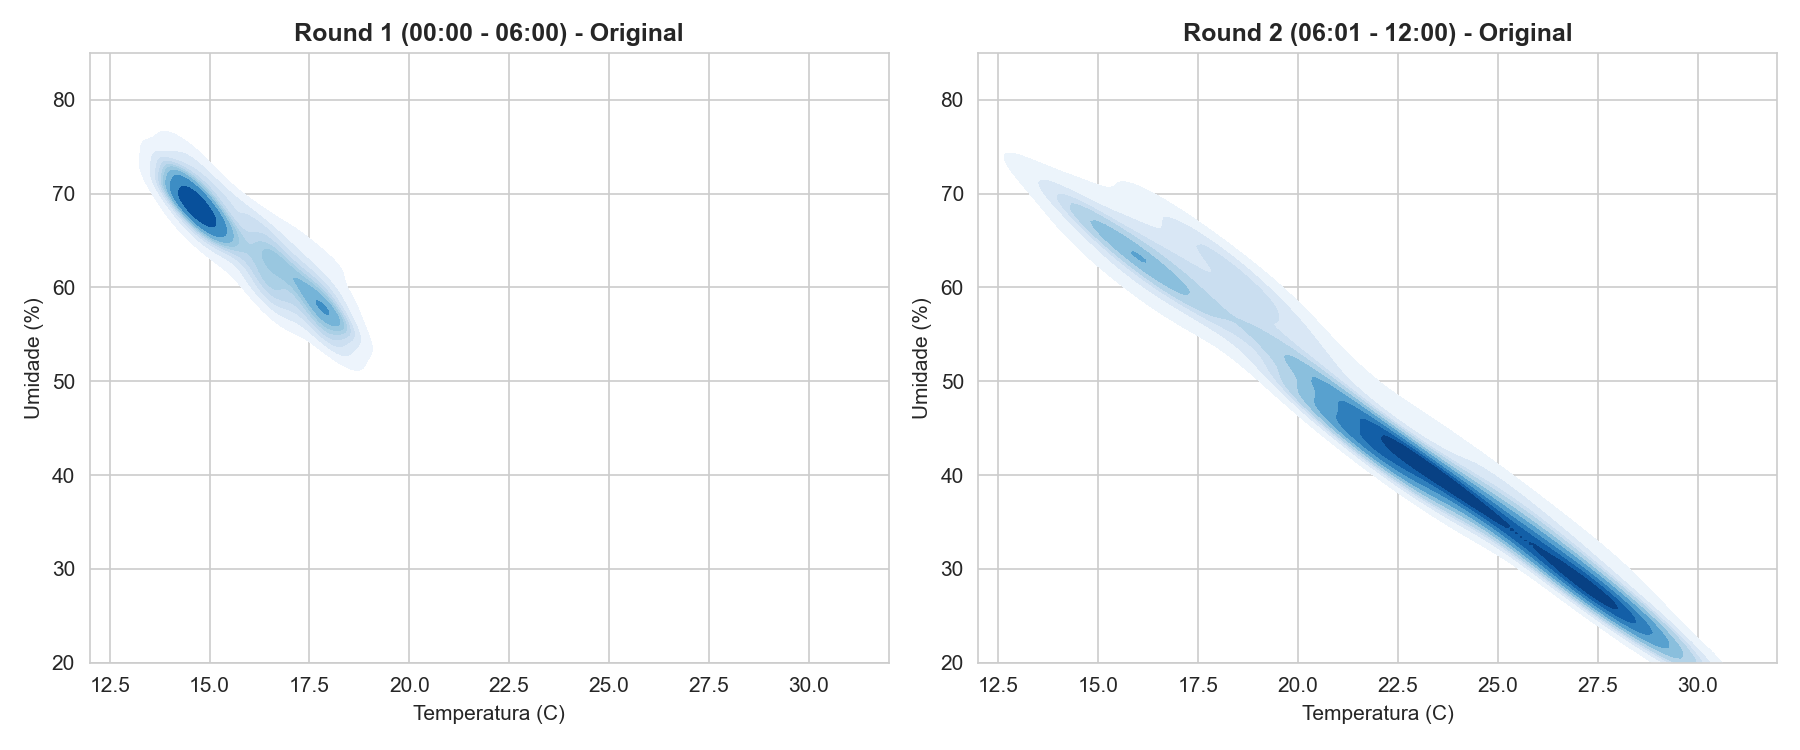
\includegraphics[width=\textwidth]{analise-experimentos/densidade_artigo_original.png}
    \caption{Dados Originais (R1 e R2)}
\end{subfigure}
\hfill
\begin{subfigure}[b]{0.48\textwidth}
    \centering
    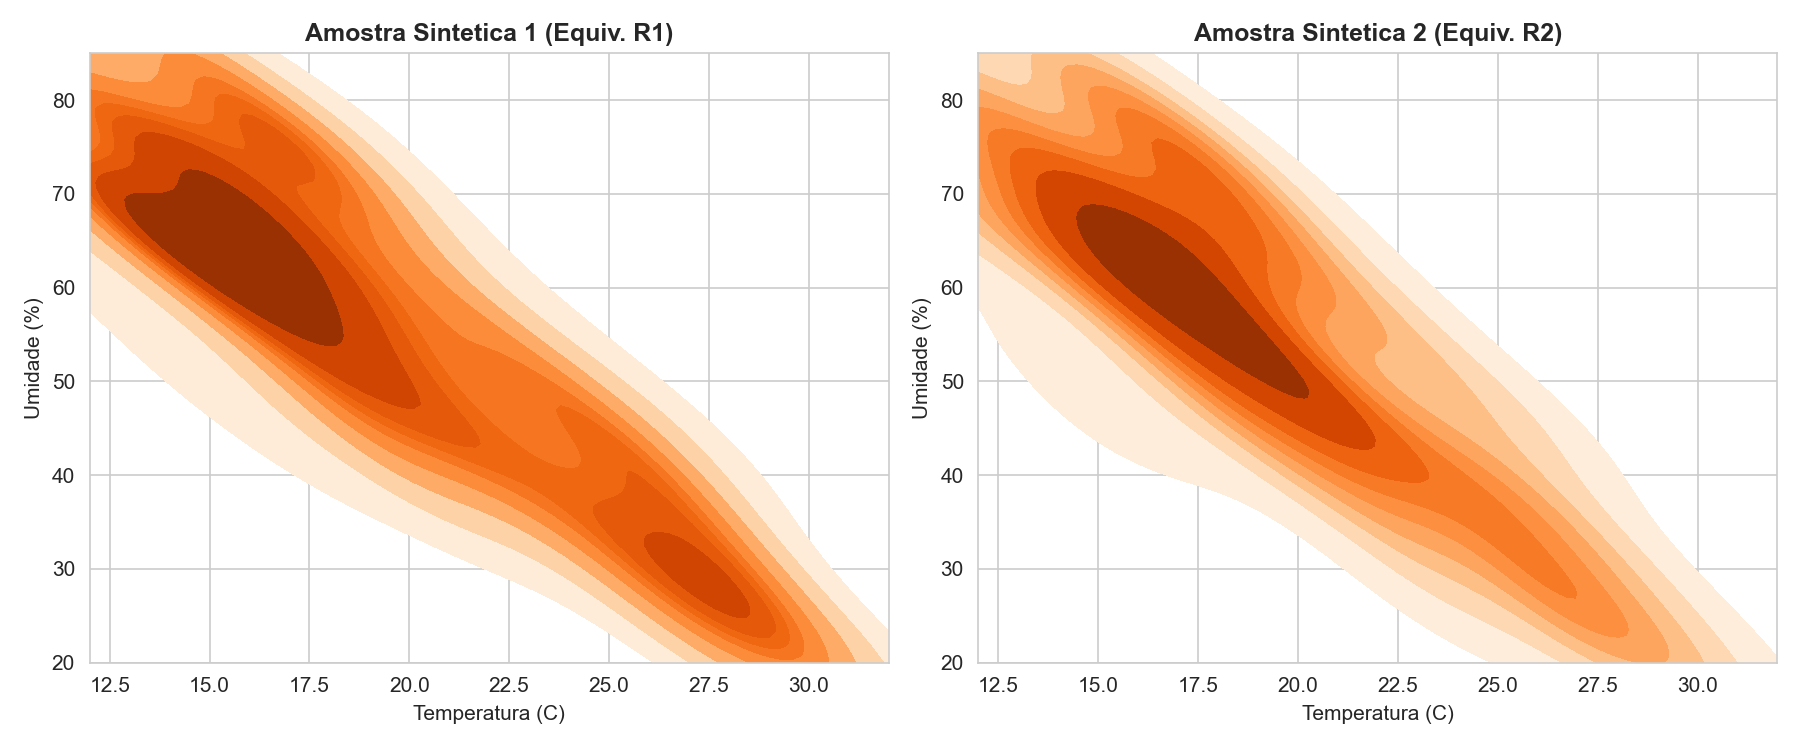
\includegraphics[width=\textwidth]{analise-experimentos/densidade_artigo_sintetico.png}
    \caption{Dados Sintéticos KDE}
\end{subfigure}
\caption{Curvas de contorno de densidade de probabilidade bidimensional}
\label{fig:densidade_original_sintetico}
\fonte{O Autor (2026)}
\end{figure}

Percebe-se que as curvas de contorno preservam os mesmos centros de adensamento térmico e de umidade relativa. As variações observadas no contorno simulado são decorrentes do kernel gaussiano suavizado ($\sigma = 0,5$), que preenche pequenos vazios na amostragem original sem distorcer o comportamento global.

Os correlogramas detalhados com a coloração dos pontos pelas classes classificadas pelo algoritmo $k$NN ($k=3$), com as curvas de densidade marginais integradas nos eixos (equivalentes à Figura 4 do artigo), são apresentados para as sub-rodadas nas Figuras~\ref{fig:correlograma_r1} e \ref{fig:correlograma_r2}.

\begin{figure}[H]
\centering
\begin{subfigure}[b]{0.48\textwidth}
    \centering
    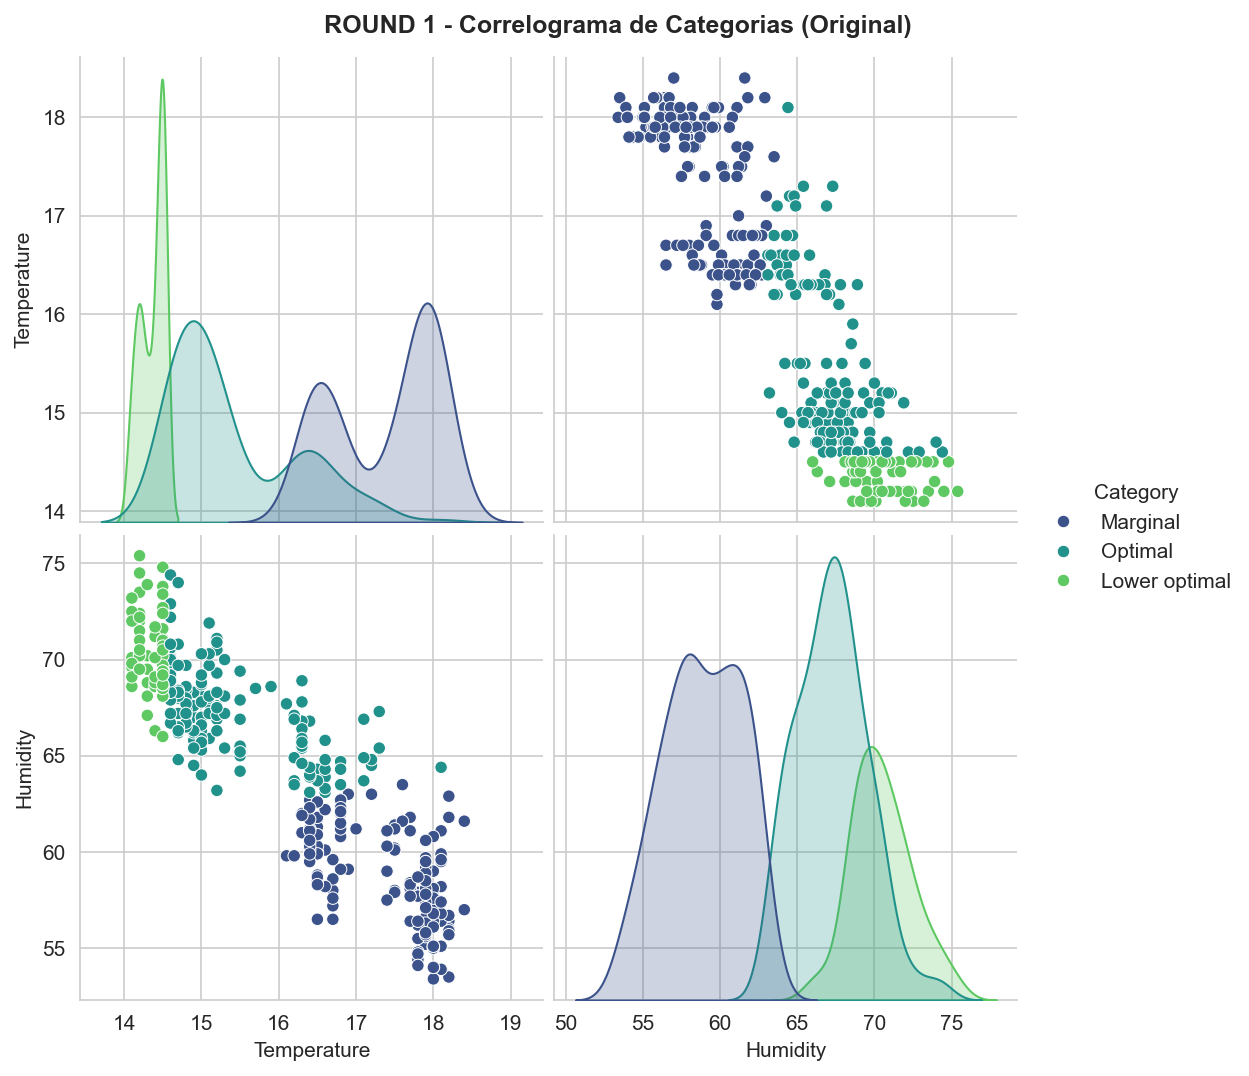
\includegraphics[width=\textwidth]{analise-experimentos/correlograma_r1_original.png}
    \caption{Round 1 - Original}
\end{subfigure}
\hfill
\begin{subfigure}[b]{0.48\textwidth}
    \centering
    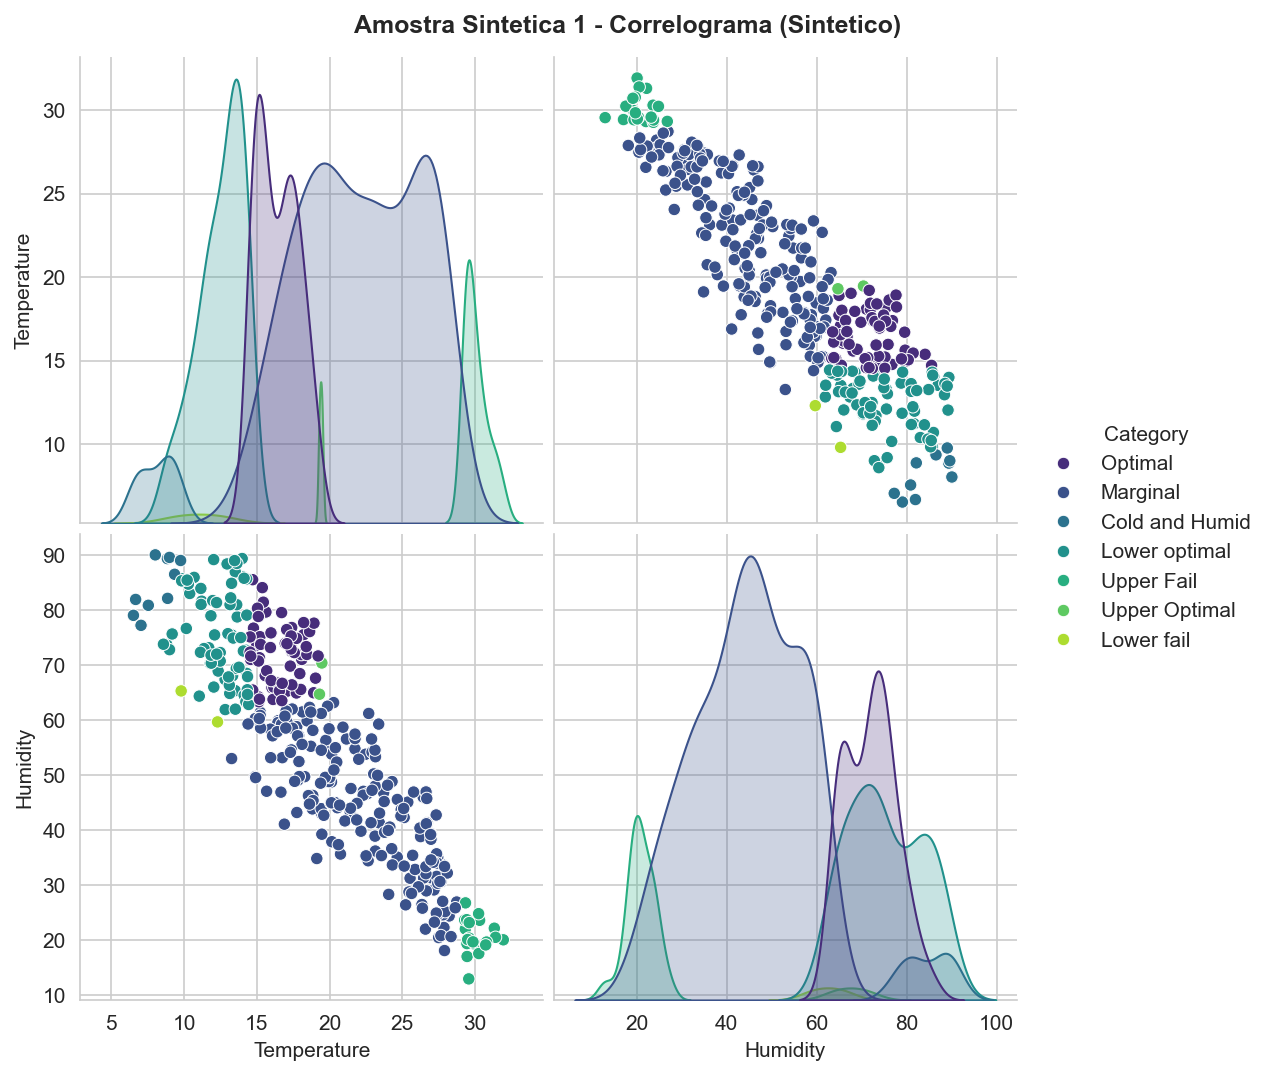
\includegraphics[width=\textwidth]{analise-experimentos/correlograma_r1_sintetico.png}
    \caption{Round 1 - Sintético}
\end{subfigure}
\caption{Correlogramas de Temperatura vs Umidade classificados por kNN (Round 1)}
\label{fig:correlograma_r1}
\fonte{O Autor (2026)}
\end{figure}

\begin{figure}[H]
\centering
\begin{subfigure}[b]{0.48\textwidth}
    \centering
    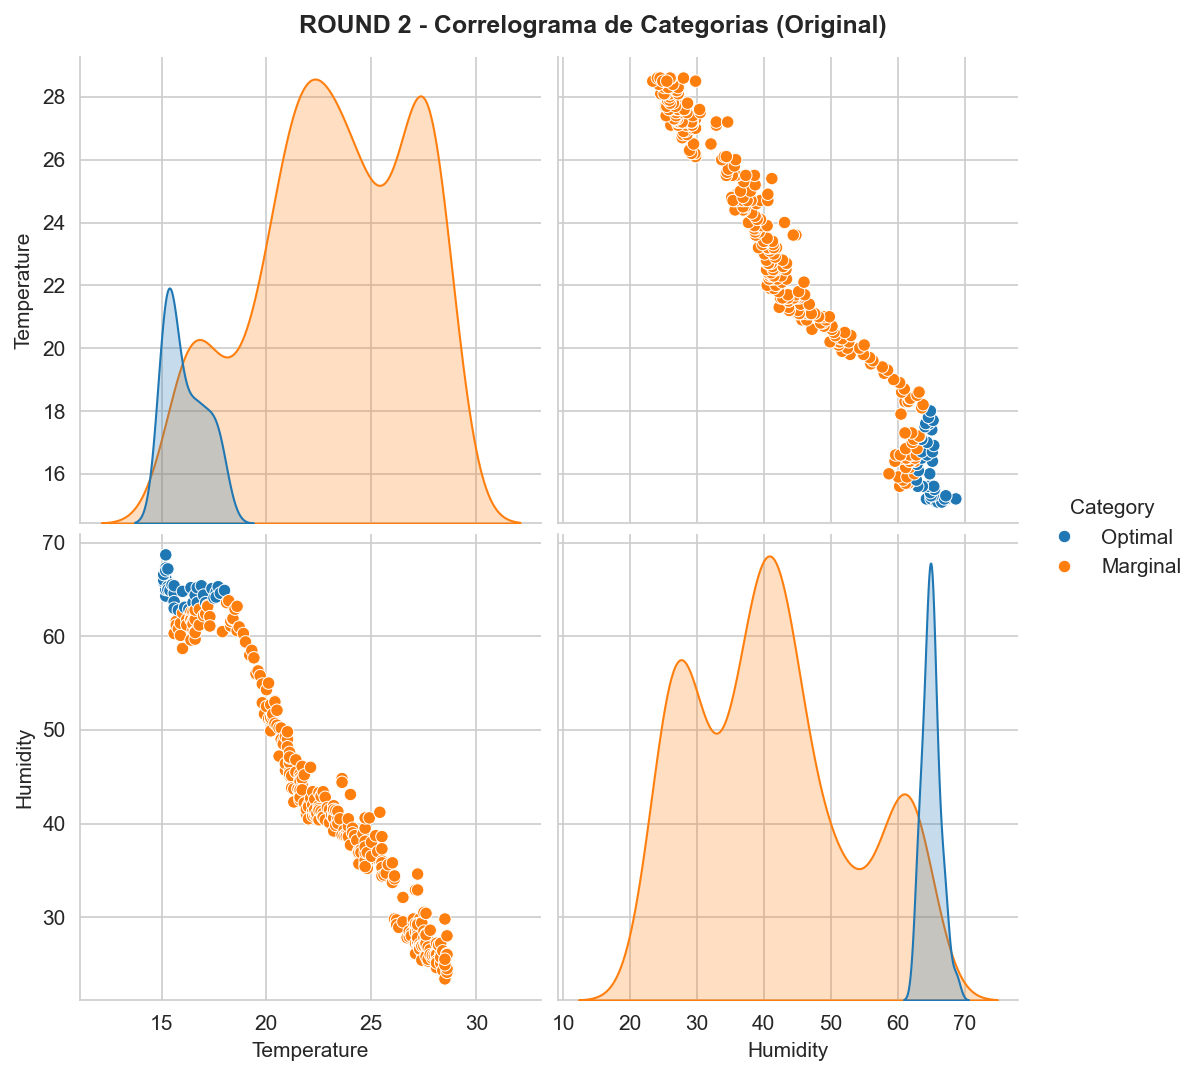
\includegraphics[width=\textwidth]{analise-experimentos/correlograma_r2_original.png}
    \caption{Round 2 - Original}
\end{subfigure}
\hfill
\begin{subfigure}[b]{0.48\textwidth}
    \centering
    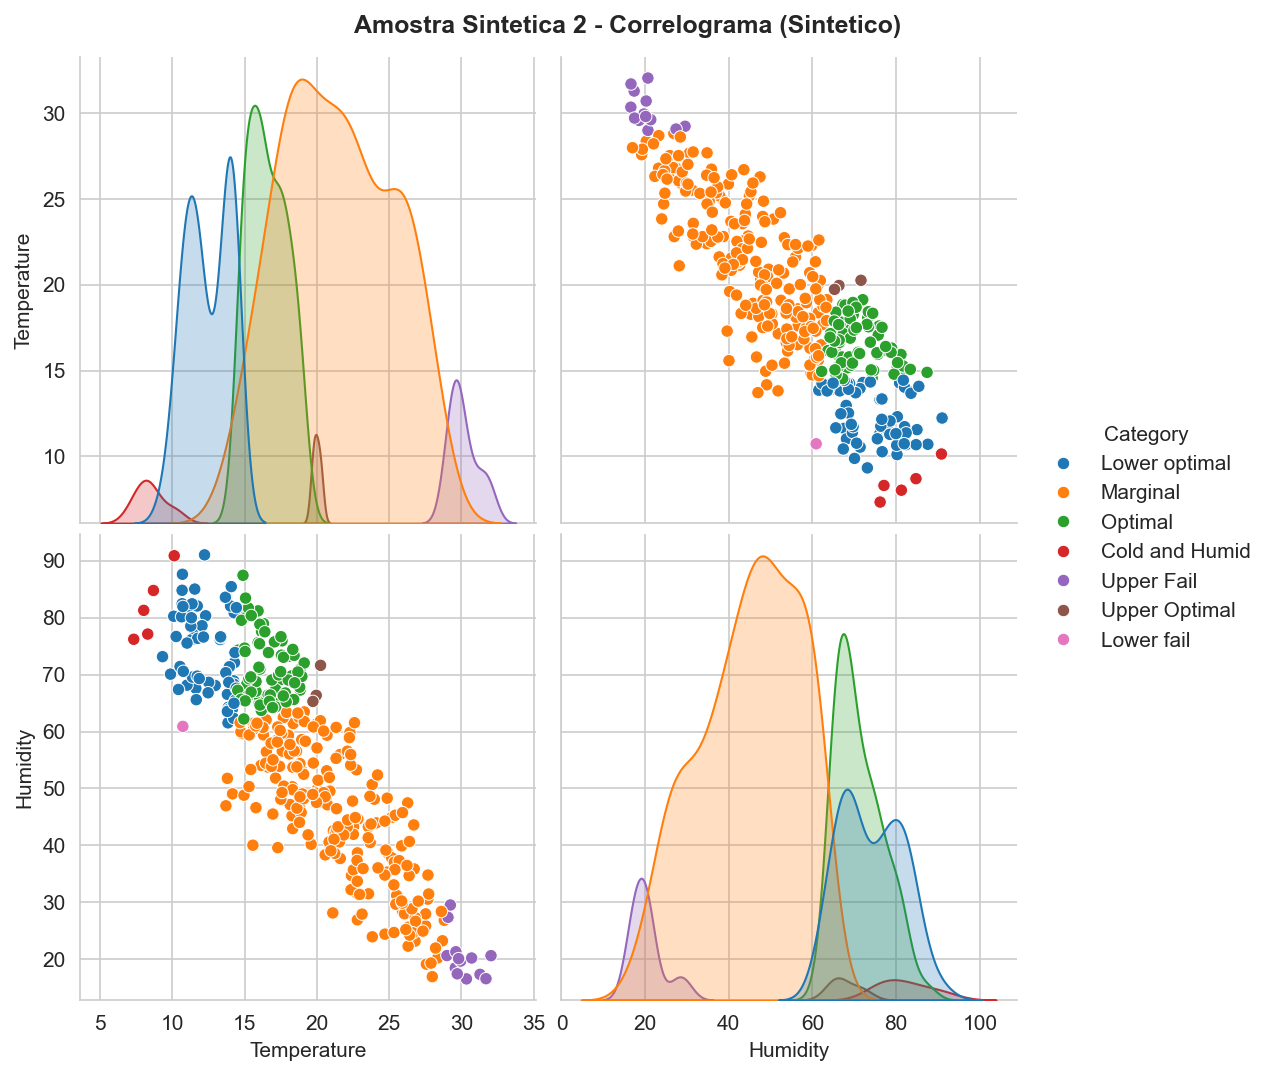
\includegraphics[width=\textwidth]{analise-experimentos/correlograma_r2_sintetico.png}
    \caption{Round 2 - Sintético}
\end{subfigure}
\caption{Correlogramas de Temperatura vs Umidade classificados por kNN (Round 2)}
\label{fig:correlograma_r2}
\fonte{O Autor (2026)}
\end{figure}

Os correlogramas mostram uma sobreposição quase perfeita das fronteiras de decisão do classificador $k$NN entre os dados reais e os dados gerados de forma estocástica. As distribuições marginais de temperatura e umidade ao longo dos eixos demonstram graficamente a similaridade atestada pelo teste KS.

Finalmente, a Figura~\ref{fig:densidade_global} apresenta a comparação global de contorno bidimensional para a base completa de dados reais e sintéticos.

\begin{figure}[H]
\centering
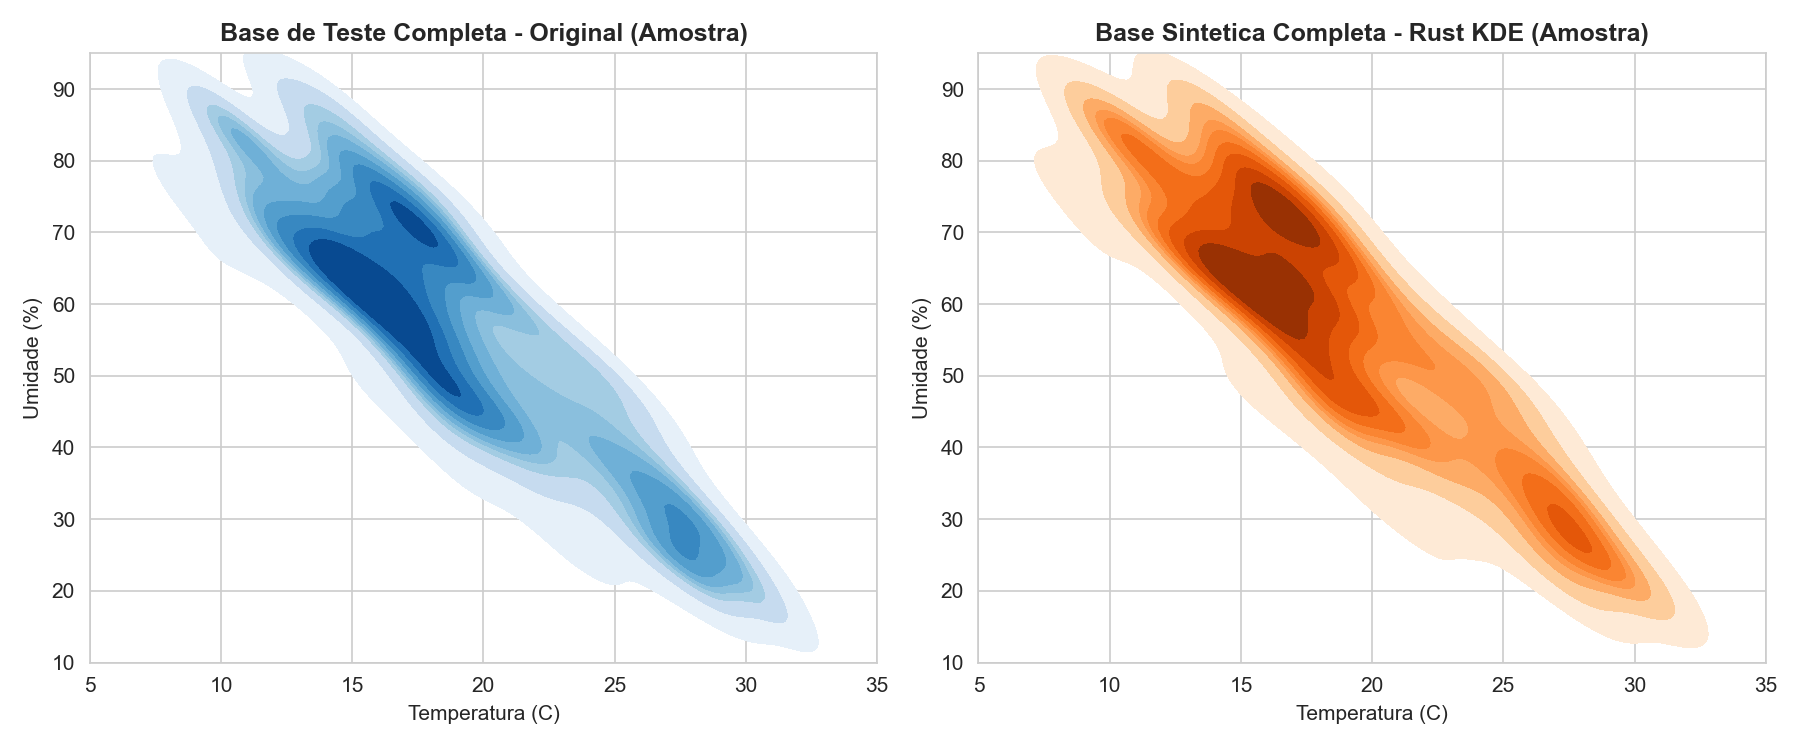
\includegraphics[width=12cm]{analise-experimentos/densidade_global_comparacao.png}
\caption{Comparação de Densidade Bidimensional Completa (Original vs Sintético)}
\label{fig:densidade_global}
\fonte{O Autor (2026)}
\end{figure}

A sobreposição visual confirma que a amostragem baseada em KDE em Rust recupera a estrutura estocástica latente dos sensores, gerando novos pontos que respeitam a física do sensor real e preenchendo as descontinuidades da grade de medição.

\section{Resultados da Compressão de Dados nos Experimentos}

Para caracterizar o impacto do empacotamento na compressão, realizou-se a segmentação da base de dados simulada de 40.000 registros em 5 cenários de lotes distintos. A Tabela~\ref{tab:simulacao_lote_detalhe} apresenta a modelagem e a partição temporal do experimento para a primeira bateria de testes (Experimento 1).

\begin{table}[H]
\centering
\caption{Detalhamento da partição dos dados em lotes no Experimento 1}
\label{tab:simulacao_lote_detalhe}
\resizebox{\textwidth}{!}{%
\begin{tabular}{ccrccc}
\toprule
\textbf{Tamanho do Lote} & \textbf{Escopo Temporal} & \textbf{Qtd. de Lotes} & \textbf{Original Acumulado (B)} & \textbf{kNN Acumulado (B)} & \textbf{RLE Acumulado (B)} \\ \midrule
6 & 30 segundos (Micro) & 6.667 & 1.856.634 & 40.000 & 70.218 \\
60 & 5 minutos & 667 & 1.850.634 & 40.000 & 68.288 \\
720 & 1 hora & 56 & 1.850.023 & 40.000 & 68.062 \\
4.320 & 6 horas & 10 & 1.849.977 & 40.000 & 67.962 \\
20.000 & ~14 horas (Metade) & 2 & 1.849.969 & 40.000 & 68.104 \\
\bottomrule
\end{tabular}%
}
\fonte{O Autor (2026)}
\end{table}

A partir do detalhamento de partição, dois fenômenos de engenharia de software e análise de dados podem ser formalizados:

\subsection{Custo de Serialização JSON e o Overhead de Colchetes}
Observa-se na Tabela~\ref{tab:simulacao_lote_detalhe} que o tamanho acumulado dos dados originais (em formato JSON bruto) diminui à medida que o tamanho do lote aumenta, passando de 1.856.634 bytes para 1.849.969 bytes (uma redução líquida de 6.665 bytes). Isso é explicado pelo custo de sintaxe da estrutura de matriz JSON (\texttt{[...]}). Cada lote processado adiciona dois caracteres sintáticos (um colchete de abertura e um de fechamento) à string serializada.
\begin{itemize}
    \item Para lote de tamanho 6, a divisão resulta em 6.667 lotes independentes, introduzindo um overhead de aproximadamente 13.334 bytes apenas em colchetes delimitadores.
    \item Para lote de tamanho 20.000, o overhead sintático cai para apenas 4 bytes no total (referente aos colchetes dos 2 lotes gerados).
\end{itemize}

\subsection{Efeito de Borda e o Lote Ideal}
O ponto de maior compressão para a técnica combinada kNN+RLE ocorreu de forma consistente no tamanho de \textbf{4.320 registros (6 horas)}, resultando em um payload de \textbf{67.962 bytes}. Isso decorre da redução do ``efeito de borda'': à medida que o tamanho do pacote aumenta, a probabilidade de uma corrida longa de categorias ser artificialmente interrompida na fronteira de divisão do lote diminui. Isso permite ao RLE formar sequências mais compactas.
Contudo, para lotes ainda maiores, como o de \textbf{20.000 registros}, o ganho é ligeiramente degradado (subindo para 68.104 bytes). Esse fenômeno decorre da representação numérica decimal das frequências no RLE. Frequências muito longas demandam mais caracteres decimais (exemplo: representar uma contagem de $12.345$ repetições da classe \texttt{Optimal} consome 6 bytes, \texttt{12345O}, enquanto contagens menores na faixa de dezenas ou centenas consomem de 2 a 3 bytes). O custo extra dos dígitos numéricos adicionais anula as vantagens marginais obtidas na eliminação das quebras de borda.

\subsection{Consistência entre Execuções Independentes}
Para validar a estabilidade estatística do gerador, os experimentos de compressão foram repetidos em três baterias completas com novos dados estocásticos gerados via KDE. A Tabela~\ref{tab:tamanhos_comprimidos} apresenta o tamanho final do payload em bytes após a codificação kNN+RLE para cada bateria.

\begin{table}[H]
\centering
\caption{Tamanhos finais após compactação kNN+RLE (Bytes)}
\label{tab:tamanhos_comprimidos}
\begin{tabular}{cccccc}
\toprule
\textbf{Tamanho do Lote} & \textbf{Experimento 1} & \textbf{Experimento 2} & \textbf{Experimento 3} & \textbf{Desvio Máx.} & \textbf{Var. \% Máx.} \\ \midrule
6 & 70.218 & 70.142 & 70.038 & 180 B & $0,25\%$ \\
60 & 68.288 & 67.982 & 68.166 & 306 B & $0,44\%$ \\
720 & 68.062 & 68.072 & 67.932 & 140 B & $0,20\%$ \\
4.320 & 67.962 & 68.194 & 68.022 & 232 B & $0,34\%$ \\
20.000 & 68.104 & 68.082 & 68.100 & 22 B & $0,03\%$ \\
\bottomrule
\end{tabular}
\fonte{O Autor (2026)}
\end{table}

A variação máxima observada entre as execuções independentes foi extremamente reduzida (abaixo de $0,44\%$). Como kNN e RLE são determinísticos, essa flutuação residual decorre unicamente da semente aleatória do gerador estocástico KDE que altera ligeiramente as coordenadas dos pontos de dados simulados nas fronteiras de decisão das classes do tomateiro, alterando pontualmente os padrões de alternância de classes. Isso comprova a elevada estabilidade estatística e reprodutibilidade do gerador.

A Tabela~\ref{tab:taxas_reducao} resume as taxas de compressão percentual obtidas para as três baterias de teste em relação à representação original serializada em JSON.

\begin{table}[H]
\centering
\caption{Taxas de redução acumuladas (kNN+RLE) em relação ao JSON original (\%)}
\label{tab:taxas_reducao}
\begin{tabular}{ccccc}
\toprule
\textbf{Tamanho do Lote} & \textbf{Experimento 1 (\%)} & \textbf{Experimento 2 (\%)} & \textbf{Experimento 3 (\%)} & \textbf{Variação Máx. (\%)} \\ \midrule
6 & $96,22\%$ & $96,22\%$ & $96,23\%$ & $0,01\%$ \\
60 & $96,31\%$ & $96,33\%$ & $96,32\%$ & $0,02\%$ \\
720 & $96,32\%$ & $96,32\%$ & $96,33\%$ & $0,01\%$ \\
4.320 & $96,33\%$ & $96,31\%$ & $96,32\%$ & $0,02\%$ \\
20.000 & $96,32\%$ & $96,32\%$ & $96,32\%$ & $0,00\%$ \\
\bottomrule
\end{tabular}
\fonte{O Autor (2026)}
\end{table}

Percebe-se que, independente do tamanho de lote utilizado e das flutuações amostrais, a taxa de redução global de dados transmitidos fica estavelmente posicionada acima de $96,2\%$. 

\section{Comparação kNN Puro vs kNN+RLE}

Uma das contribuições mais relevantes deste estudo emerge da comparação direta entre o uso de apenas a classificação kNN (kNN Puro) e a combinação de classificação com codificação de corrida (kNN+RLE). A Tabela~\ref{tab:pure_vs_rle} traz a comparação média das taxas de redução.

\begin{table}[H]
\centering
\caption{Comparação de redução: kNN Puro vs kNN+RLE}
\label{tab:pure_vs_rle}
\begin{tabular}{cccl}
\toprule
\textbf{Tamanho do Lote} & \textbf{Redução kNN Puro (\%)} & \textbf{Redução kNN+RLE (\%)} & \textbf{Melhor Opção} \\ \midrule
6 (30 s) & $97,85\%$ (40 KB) & $96,22\%$ (70 KB) & \textbf{kNN Puro} ($+1,63\%$) \\
60 (5 min) & $97,84\%$ (40 KB) & $96,32\%$ (68 KB) & \textbf{kNN Puro} ($+1,52\%$) \\
720 (1 h) & $97,84\%$ (40 KB) & $96,31\%$ (68 KB) & \textbf{kNN Puro} ($+1,53\%$) \\
4.320 (6 h) & $97,84\%$ (40 KB) & $96,32\%$ (68 KB) & \textbf{kNN Puro} ($+1,52\%$) \\
20.000 (14 h) & $97,84\%$ (40 KB) & $96,32\%$ (68 KB) & \textbf{kNN Puro} ($+1,52\%$) \\
\bottomrule
\end{tabular}
\fonte{O Autor (2026)}
\end{table}

Os dados revelam uma constatação contra-intuitiva: **o kNN Puro comprime mais e gera payloads menores do que o kNN+RLE em todas as configurações**. O kNN Puro reduziu o arquivo final para estáveis 40 KB, enquanto o RLE resultou em arquivos entre 68 KB e 70 KB.

\subsection{Discussão sobre a Ineficiência do RLE}

Esse comportamento deve-se a dois fatores principais decorrentes do alfabeto de símbolos curto do classificador $k$NN:

\begin{enumerate}
    \item **Fenômeno de Expansão de Símbolo Único**:
    O kNN converte cada par de leituras físicas em uma string de um caractere (por exemplo, `O` para *Optimal*). Portanto, 40.000 leituras correspondem a 40.000 caracteres de texto puro, ocupando exatamente 40.000 bytes.
    Quando o RLE atua, ele agrupa caracteres repetidos na estrutura `<frequência><categoria>` (ex: `3O`). Para leituras com baixa repetição consecutiva (comprimento de corrida $C = 1$), o RLE codifica a ocorrência como `1O` (ocupando **2 bytes**, o que representa uma expansão de $100\%$ do tamanho original de $1$ byte).
    
    \item **Oscilação Natural do Sensor Físico (Ruído de Fronteira)**:
    Como temperatura e umidade flutuam continuamente sob efeito de ruído físico na bacia de captação dos sensores, os dados próximos aos limites de decisão do classificador $k$NN oscilam constantemente de classe (por exemplo, alternando entre `O`, `P` e `S` a cada minuto). Essas alternâncias de alta frequência rompem a homogeneidade das corridas contíguas. 
    A grande quantidade de corridas de comprimento unitário ou muito curtas geradas pela variabilidade dos dados causa uma expansão de volume que anula a economia de espaço proporcionada pelas raras corridas longas, resultando em um payload total acumulado de 68 KB a 70 KB para o RLE contra os 40 KB estáveis do kNN Puro.
\end{enumerate}

Essa análise revela que a compactação RLE é inadequada se a codificação do kNN já foi previamente otimizada para 1 caractere de comprimento. O RLE só apresentaria vantagem se o kNN puro exportasse rótulos textuais completos (como `"Optimal"`, `"Upper Marginal"`), caso em que o custo de strings de 7 a 15 bytes justificaria o overhead de adicionar contadores.

% ==========================================================
\chapter{CONCLUSÃO}
\label{cap:conclusao}
% ==========================================================

Este trabalho apresentou uma abordagem robusta e eficiente para a computação em névoa aplicada à IoT agrícola. A migração dos algoritmos de classificação kNN e compressão de dados para Rust compilado em WebAssembly demonstrou a viabilidade de implantar soluções analíticas de alta segurança e portabilidade em gateways de borda reais com baixíssimo consumo de recursos computacionais.

O simulador estocástico desenvolvido em Rust/WASM, fundamentado na Estimativa de Densidade por Kernel (KDE) e na Transformada de Box-Muller, comprovou ser uma ferramenta científica valiosa para modelar e gerar de forma altamente precisa dados sintéticos de sensores locais. Os testes Kolmogorov-Smirnov e a correlação de Pearson atestaram a excelente representatividade física dos dados simulados.

Os experimentos de compressão revelaram a ineficiência prática da combinação kNN+RLE em relação ao kNN puro quando o formato do status agronômico já é otimizado para caracteres únicos de 1 byte. Esse resultado contraria suposições teóricas comuns de projetos de transmissão IoT e serve como uma diretriz empírica crucial para projetistas de sistemas de monitoramento agrícola.

Como trabalhos futuros, propõe-se a validação em campo utilizando gateways LoRaWAN físicos baseados em arquiteturas ARM de baixo custo executando WasmEdge. Sugere-se também a investigação de algoritmos de classificação adaptativos que ajustem dinamicamente o valor de $k$ com base no nível de bateria disponível nos nós sensores, e a aplicação de classificadores robustos a ruídos de fronteira de modo a minimizar as oscilações de classificação que degradam a eficiência da codificação temporal.

% ----------------------------------------------------------
% REFERÊNCIAS
% ----------------------------------------------------------
\begin{thebibliography}{99}

\bibitem{ribeiro2020nearest}
RIBEIRO JUNIOR, L. A. S.; PRATI, R. C.; BIANCHI, R. A. C.; KAMIENSKI, C. A.
A Nearest Neighbors based Data Filter for Fog Computing in IoT Smart Agriculture.
In: IEEE INTERNATIONAL WORKSHOP ON METROLOGY FOR AGRICULTURE AND FORESTRY (MetroAGriFor), 2020, Trento.
\textit{Proceedings\dots} Washington: IEEE, 2020. p. 194--198.
DOI: 10.1109/MetroAGriFor50201.2020.9307482.

\bibitem{ekman1971constants}
EKMAN, P.; FRIESEN, W. V.
Constants across cultures in the face and emotion.
\textit{Journal of Personality and Social Psychology}, v. 17, n. 2, p. 124--129, 1971.

\bibitem{ekman1978facial}
EKMAN, P.; FRIESEN, W. V.
\textbf{Facial Action Coding System}: a technique for the measurement of facial movement.
Palo Alto: Consulting Psychologists Press, 1978.

\bibitem{goodfellow2013challenges}
GOODFELLOW, I. J. et al.
Challenges in representation learning: a report on three machine learning contests.
In: INTERNATIONAL CONFERENCE ON NEURAL INFORMATION PROCESSING, 2013, Daegu.
\textit{Proceedings\dots} Berlin: Springer, 2013. p. 117--124.

\bibitem{lugaresi2019mediapipe}
LUGARESI, C. et al.
{MediaPipe}: a framework for building perception pipelines.
In: ACM MULTIMEDIA CONFERENCE, 2019, Nice.
\textit{Proceedings\dots} New York: ACM, 2019. p. 1098--1101.

\bibitem{mcinnes2018umap}
MCINNES, L.; HEALY, J.; MELVILLE, J.
{UMAP}: Uniform Manifold Approximation and Projection for dimension reduction.
\textit{arXiv preprint arXiv:1802.03426}, 2018.

\bibitem{serengil2020lightface}
SERENGIL, S. I.; OZPINAR, A.
LightFace: a hybrid deep face recognition framework.
In: INNOVATIONS IN INTELLIGENT SYSTEMS AND APPLICATIONS CONFERENCE, 2020, Istanbul.
\textit{Proceedings\dots} Washington: IEEE, 2020. p. 23--27.

\bibitem{szeliski2010computer}
SZELISKI, R.
\textbf{Computer vision}: algorithms and applications.
London: Springer, 2010.

\bibitem{wu2023yunet}
WU, W.; PENG, H.; YU, S.
{YuNet}: a tiny millisecond-level face detector.
\textit{CAAI Transactions on Intelligence Technology}, v. 8, n. 4, p. 1155--1165, 2023.

\bibitem{fastapi2019}
RAMÍREZ, S.
\textbf{FastAPI}: a modern, fast (high-performance), web framework for building APIs.
2019. Disponível em: \url{https://fastapi.tiangolo.com}. Acesso em: maio 2026.

\end{thebibliography}

% --- Apêndices ---
\begin{apendicesenv}

\chapter{ESTRUTURA DO PROJETO DE SENSORES E NÉVOA}

A estrutura de diretórios do ecossistema PGC-Rust está organizada da seguinte forma:

\begin{lstlisting}[language=bash, caption={Estrutura de diretórios do PGC-Rust}]
pgc-rust/
├── processador/             # Modulo da Nevoa (WASM)
│   ├── Cargo.toml
│   └── src/
│       └── main.rs          # Algoritmo kNN, RLE e Gerador KDE
├── simulador/               # Componente do dispositivo IoT (Thing)
│   ├── Cargo.toml
│   └── src/
│       └── main.rs
├── receiver/                # Módulo da Nuvem (Cloud)
│   ├── Cargo.toml
│   └── src/
│       └── main.rs
├── gerador-de-dados/        # Scripts auxiliares e validacao estocastica
│   ├── gerar_dados_sinteticos.py
│   ├── gerar_graficos_artigo.py  # Gerador de graficos de contorno
│   └── validar_dados_rust.py    # Executa teste KS e Pearson
├── analise-experimentos/    # Resultados dos experimentos 1, 2 e 3
│   ├── experimento-1/
│   │   └── dados_sinteticos_gerados_rust.csv
│   ├── densidade_artigo_original.png
│   ├── densidade_artigo_sintetico.png
│   ├── correlograma_r1_original.png
│   └── correlograma_r2_sintetico.png
├── entrada.csv              # Base de dados original
└── run_experiments.sh       # Executa bateria de testes do PGC
\end{lstlisting}

\chapter{MODELO DOS DADOS SERIALIZADOS (JSON)}

A seguir é apresentado o formato JSON de serialização das estatísticas de compressão exportadas pelo processador em modo lote:

\begin{lstlisting}[language=Python, caption={Modelo JSON de Estatísticas de Compressão}]
{
  "tamanho_lote": 20000,
  "total_registros": 40000,
  "bytes_originais": 1856634,
  "bytes_knn_puro": 40000,
  "bytes_knn_rle": 68104,
  "taxa_reducao_knn": 97.8455,
  "taxa_reducao_rle": 96.3318,
  "experimentos": [
    {
      "lote_id": 0,
      "tamanho": 20000,
      "frequencias_classes": {
        "Optimal": 25421,
        "Upper Optimal": 12102,
        "Marginal": 2477
      }
    }
  ]
}
\end{lstlisting}

\end{apendicesenv}

\end{document}
